\documentclass[11pt,a4paper]{article}

\newcommand{\Title}{Supplementary Information for "Multipole Modeling for Magnetic Microscopy Constrained by Euler Deconvolution"}

\newcommand{\TitleShort}{Multipoles Inversion from Euler Deconvolution}

\newcommand{\Year}{2026}
\newcommand{\SubmittedOn}{2026/08/07}
\newcommand{\PublishedOn}{2026/08/07}

\newcommand{\AuthorShort}{Souza-Junior \textit{et al.}}
\newcommand{\Authors}{%
Gelson F. Souza-Junior\textsuperscript{1,2*},
Ualisson D. Bellon\textsuperscript{3*},
Leonardo Uieda\textsuperscript{1},
Ricardo I. F. Trindade\textsuperscript{1},
Roger R. Fu\textsuperscript{2},
Wyn Williams\textsuperscript{3}, and
Arthur Siqueira-Macedo\textsuperscript{1}
}
\newcommand{\Emailgelson}{gelson.ferreiral@iag.usp.br}
\newcommand{\Emailualisson}{ualisson.bellon@ed.ac.uk}

\newcommand{\Corresponding}{%
  Corresponding authors: Gelson F. Souza-Junior <\href{mailto:\Emailgelson}{\Emailgelson}> \\
~~~~~~~~~~~~~~~~~~~~~~~~~~~~~~~~Ualisson D. Bellon <\href{mailto:\Emailualisson}{\Emailualisson}>
}
\newcommand{\Affiliations}{%
  \textsuperscript{1} Universidade de São Paulo, Brazil;
  \textsuperscript{2} Harvard University, USA;
  \textsuperscript{3} University of Edinburgh, UK;
  \textsuperscript{*} Co-first authorship;
}

\newcommand{\Journal}{Journal of Geophysical Research: Solid Earth}
\newcommand{\JournalDOI}{YYYYY/YYYYYYY}
\newcommand{\PreprintDOI}{XXXXX/XXXXXXX}
\newcommand{\ArchiveDOI}{10.5281/zenodo.20446907}
\newcommand{\GitHubRepository}{compgeolab/micromag-spherical-harmonic}

\newcommand{\Keywords}{%
  keyword1; keyword2; keyword3;
}

\usepackage[utf8]{inputenc}
\usepackage[TU]{fontenc}
\usepackage[english]{babel}
\usepackage{geometry}
\usepackage{booktabs}
\usepackage{amsmath}
\usepackage{amssymb}
\usepackage{graphicx}
\usepackage{hyperref}
\usepackage{fancyhdr}
\usepackage{orcidlink}
\usepackage{microtype}
\usepackage{siunitx}
\usepackage{fontawesome5}
\usepackage{academicons}
\usepackage{anyfontsize}
\usepackage{setspace}
\usepackage{lastpage}
\usepackage{lipsum}
\usepackage{ragged2e}
\usepackage{soul}
\usepackage{natbib}

\definecolor{mediumblue}{HTML}{2060c2}

\hypersetup{
    colorlinks,
    allcolors=mediumblue,
    pdftitle={\Title},
    pdfauthor={\AuthorShort},
    breaklinks=true,
}

\geometry{margin=0.75in}

% Redefine the numbering to the supplementary format (S1, S2...)
\renewcommand{\thefigure}{S\arabic{figure}}
\renewcommand{\thetable}{S\arabic{table}}

\begin{document}

\thispagestyle{plain}

\begin{FlushLeft}
  \begin{spacing}{2}
    {\LARGE\bfseries \Title}
  \end{spacing}
  {\color{lightgray}\hrule height 1.5pt}
  \vspace{0.3cm}
  \Authors
  \\[0.2cm]
  {\footnotesize \Affiliations}
  \newline
  {\footnotesize \Corresponding}
  \\[0.2cm]
  {\footnotesize
    Received in original form on \SubmittedOn.
    %Published in final form on \PublishedOn.
  }
\end{FlushLeft}

\newpage
The micromagnetic models are fully detailed below (Table~\ref{tab:models_si}), providing a complete specification of all 20 simulation geometries, material parameters, discretization details, and resulting net magnetic moments. We assigned the temperature-dependent magnetic parameters of magnetite at $20\,^\circ\mathrm{C}$ to all minimizations, namely a saturation magnetization of $M_s = 4.825 \times 10^5$~A/m \citep{Pauthenet-1951}, first- and second-order magnetocrystalline anisotropy constants of $K_1 = -1.304 \times 10^4$~J/m$^3$ and $K_2 = -3.154 \times 10^3$~J/m$^3$, respectively \citep{Fletcher-1974}, and an exchange stiffness of $A_{\mathrm{ex}} = 1.344 \times 10^{-11}$~J/m \citep{Heider-1988}. The particles were discretized using tetrahedral elements with an average mesh resolution of $9$~nm. Models were initialized from random magnetic configurations, and 100 independent initial states were calculated for each particle. The lowest-energy state among these 100 minimizations was retained for analysis. All particles were relaxed without an externally applied magnetic field. The exact dimensions, shapes, and net magnetic moment components ($m_x$, $m_y$, $m_z$) for each model configuration are listed below.

\begin{table}[!htbp]
\centering
\caption{Complete specification of the 20 micromagnetic particle models, including shapes, exact dimensions, and resulting net magnetic moments.}
\label{tab:models_si}
\begin{tabular}{llcccc}
\toprule
\textbf{Model} & \textbf{Shape} & \textbf{Dimensions ($\mu$m)} &
$\mathbf{m_x}$ (A$\cdot$m$^2$) &
$\mathbf{m_y}$ (A$\cdot$m$^2$) &
$\mathbf{m_z}$ (A$\cdot$m$^2$) \\
\midrule
eps0 & Sphere & $R = 0.025$ &
$1.73 \times 10^{-17}$ &
$1.73 \times 10^{-17}$ &
$1.69 \times 10^{-17}$ \\

eps1 & Sphere & $R = 0.050$ &
$5.33 \times 10^{-17}$ &
$-5.48 \times 10^{-17}$ &
$5.49 \times 10^{-17}$ \\

eps2 & Sphere & $R = 0.250$ &
$-3.37 \times 10^{-16}$ &
$3.37 \times 10^{-16}$ &
$-3.37 \times 10^{-16}$ \\

eps3 & Sphere & $R = 0.375$ &
$6.97 \times 10^{-16}$ &
$6.95 \times 10^{-16}$ &
$-6.96 \times 10^{-16}$ \\

eps4 & Sphere & $R = 0.500$ &
$-1.04 \times 10^{-15}$ &
$-1.04 \times 10^{-15}$ &
$-1.04 \times 10^{-15}$ \\

\midrule

eps5 & Prolate & $a = 0.025, b = c = 0.013$ &
$-6.81 \times 10^{-18}$ &
$4.92 \times 10^{-20}$ &
$-6.62 \times 10^{-20}$ \\

eps6 & Prolate & $a = 0.050, b = c = 0.025$ &
$-6.07 \times 10^{-17}$ &
$7.09 \times 10^{-20}$ &
$-3.59 \times 10^{-20}$ \\

eps7 & Prolate & $a = 0.250, b = c = 0.125$ &
$4.64 \times 10^{-16}$ &
$7.23 \times 10^{-17}$ &
$1.87 \times 10^{-18}$ \\

eps8 & Prolate & $a = 0.375, b = c = 0.188$ &
$-6.68 \times 10^{-16}$ &
$1.12 \times 10^{-16}$ &
$2.66 \times 10^{-18}$ \\

eps9 & Prolate & $a = 0.500, b = c = 0.250$ &
$8.80 \times 10^{-16}$ &
$-1.77 \times 10^{-16}$ &
$-1.79 \times 10^{-18}$ \\

\midrule

eps10 & Oblate & $a = b = 0.025, c = 0.013$ &
$-1.02 \times 10^{-17}$ &
$-1.02 \times 10^{-17}$ &
$3.52 \times 10^{-20}$ \\

eps11 & Oblate & $a = b = 0.050, c = 0.025$ &
$-8.74 \times 10^{-17}$ &
$-8.73 \times 10^{-17}$ &
$-7.62 \times 10^{-21}$ \\

eps12 & Oblate & $a = b = 0.250, c = 0.125$ &
$2.54 \times 10^{-18}$ &
$-4.70 \times 10^{-19}$ &
$4.89 \times 10^{-17}$ \\

eps13 & Oblate & $a = b = 0.375, c = 0.188$ &
$-1.85 \times 10^{-17}$ &
$-2.00 \times 10^{-18}$ &
$-1.25 \times 10^{-16}$ \\

eps14 & Oblate & $a = b = 0.500, c = 0.250$ &
$1.72 \times 10^{-17}$ &
$-7.83 \times 10^{-17}$ &
$3.58 \times 10^{-16}$ \\

\midrule

eps15 & Euhedral & $E_{max} = 0.05$ &
$1.83 \times 10^{-17}$ &
$1.82 \times 10^{-17}$ &
$1.82 \times 10^{-17}$ \\

eps16 & Euhedral & $E_{max} = 0.10$ &
$-4.81 \times 10^{-17}$ &
$4.88 \times 10^{-17}$ &
$-4.91 \times 10^{-17}$ \\

eps17 & Euhedral & $E_{max} = 0.50$ &
$-2.99 \times 10^{-16}$ &
$-2.99 \times 10^{-16}$ &
$2.99 \times 10^{-16}$ \\

eps18 & Euhedral & $E_{max} = 0.75$ &
$5.03 \times 10^{-16}$ &
$5.03 \times 10^{-16}$ &
$5.02 \times 10^{-16}$ \\

eps19 & Euhedral & $E_{max} = 1.00$ &
$-7.36 \times 10^{-16}$ &
$-7.37 \times 10^{-16}$ &
$7.31 \times 10^{-16}$ \\

\bottomrule
\end{tabular}
\end{table}

\clearpage

To assess the robustness of the micromagnetic relaxation procedure to variations in the numerical damping parameter, we evaluated two complementary misfit measures for all particle models. The first quantifies the angular difference between the magnetic moment obtained from the first-order spherical-harmonic expansion evaluated on the spherical shell described in the main text and the net magnetic moment of the corresponding synthetic model. This angular misfit is reported in degrees in panel (a). The second quantifies the relative difference in magnetic-moment magnitude between the first-order spherical-harmonic estimate and the net magnetic moment of the synthetic model, expressed as a percentage in panel (b). Together, these metrics assess the sensitivity of both the recovered magnetic-moment direction and magnitude to variations in the numerical damping parameter.

\begin{figure}[htbp]
\centering
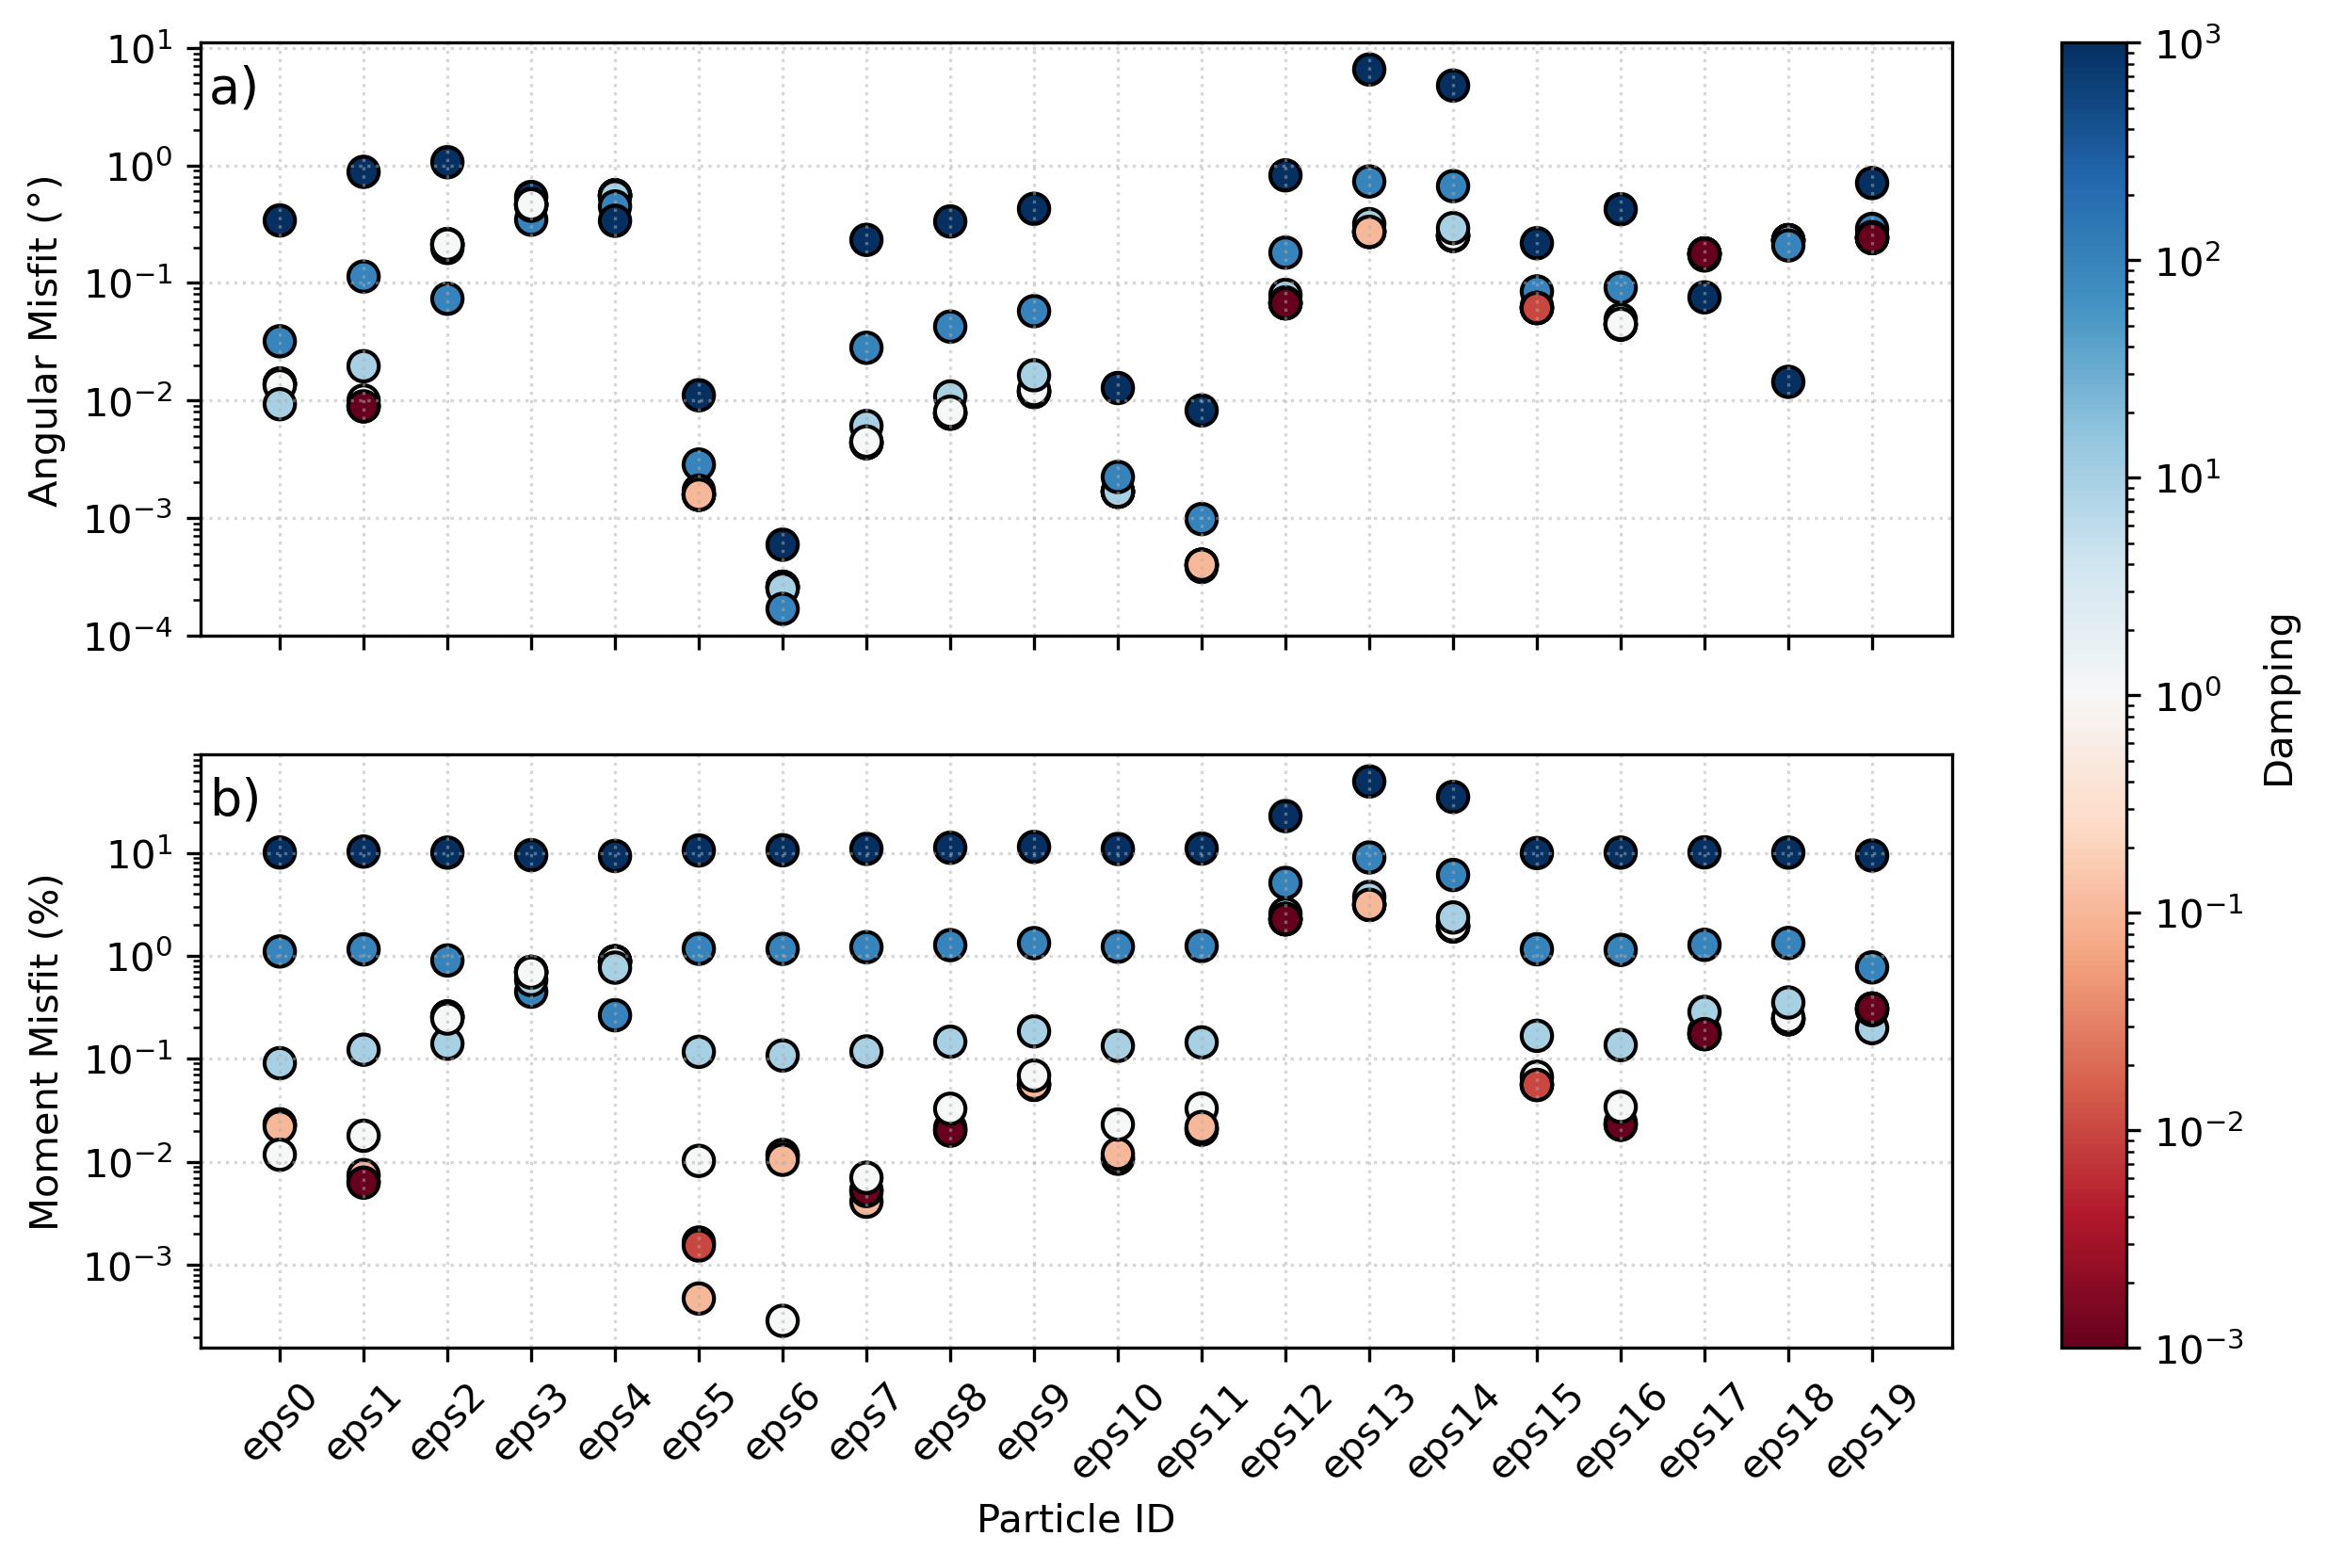
\includegraphics[width=1\textwidth]{figures/damping_sensitivity_analysis.png}
\caption{Sensitivity of the recovered magnetic moment to the numerical damping parameter for all synthetic particle models. (a) Angular misfit, in degrees, between the first-order spherical-harmonic estimate obtained on the spherical shell described in the main text and the net magnetic moment of the corresponding synthetic model. (b) Relative magnetic-moment misfit, expressed as a percentage, between the magnitudes of the first-order spherical-harmonic estimate and the net magnetic moment of the corresponding synthetic model.}
\label{fig:damping}
\end{figure}

\clearpage

For completeness, we provide here the full comparison of inversion performance across all particle geometries, sizes, inversion strategies, and sensor heights. The corresponding figure in the main text was simplified to improve readability by omitting the intermediate particle sizes for each geometry and the linear inversion results. The complete set of results, including these intermediate sizes and the linear inversion models, is shown in Figure~\ref{fig:model_comp}.

\begin{figure}[htbp]
\centering
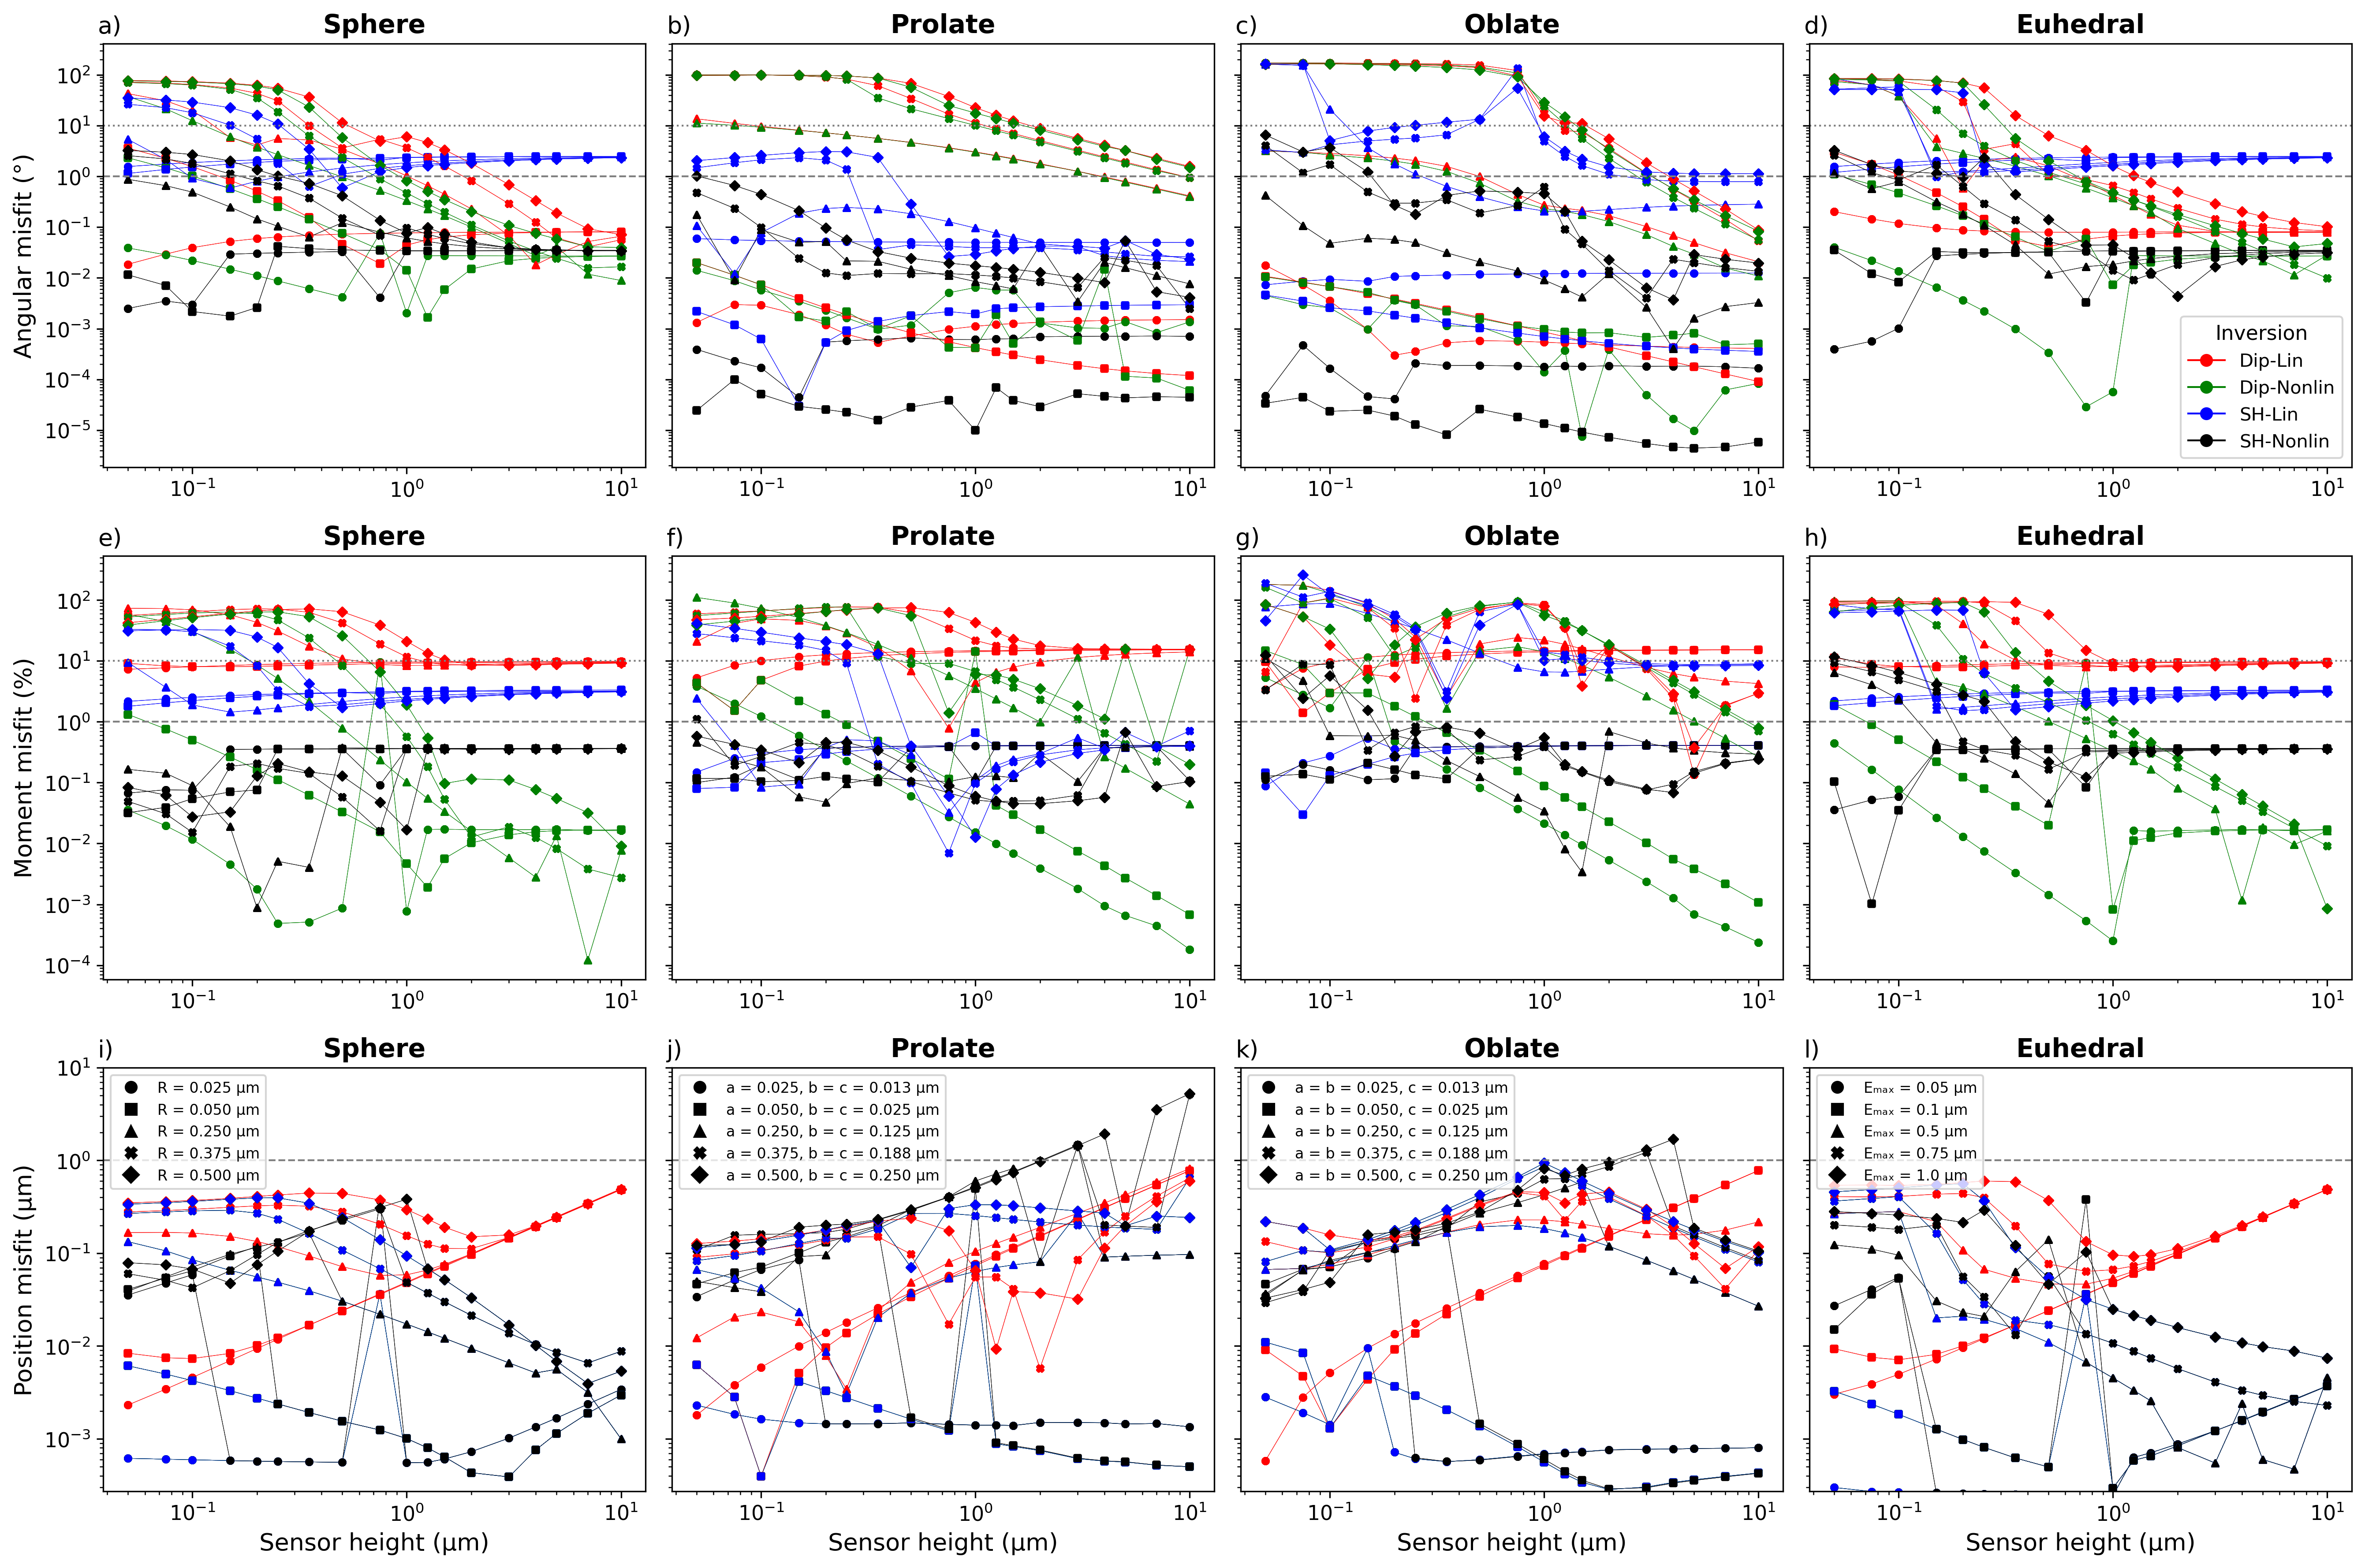
\includegraphics[width=1.\textwidth]{paper/figures/model_comparison_supplementary.png}
\caption{
Complete comparison of inversion performance for the synthetic micromagnetic particle models as a function of sensor-to-sample distance. Columns correspond to spherical, prolate, oblate, and euhedral particle geometries (left to right), while rows show angular, magnetic-moment, and position misfits (top to bottom). Each panel includes all particle sizes considered for the corresponding geometry. Colors distinguish the inversion strategies: linear dipole (Dip-Lin, red), nonlinear dipole (Dip-Nonlin, green), linear spherical-harmonic (SH-Lin, blue), and nonlinear spherical-harmonic (SH-Nonlin, black). Marker symbols identify the different particle sizes or characteristic dimensions within each geometry, as indicated in the panel legends. Horizontal dashed lines indicate the reference thresholds used for performance assessment.
}
\label{fig:model_comp}
\end{figure}


\clearpage
\bibliographystyle{apalike-doi}
\bibliography{references}
\end{document}
